%//==============================--@--===========================
\subsubsection[5.3 Multiple Access Links and Protocols]{\hspace*{0.075 em}\raisebox{0.2 em}{$\pmb{\drsh}$} Multiple Access Links and Protocols}

Broadcast links allow multiple nodes to send and receive data on a shared channel. Multiple access protocols coordinate transmissions to minimize collisions and optimize throughput; they widely used in various network settings such as wired and wireless access networks, satellite networks, and local area networks (LANs).  The three main categories of these protocols are channel partitioning, random access, and taking-turns protocols.

\vspace{1em}
\noindent An ideal multiple access protocol should have the following characteristics:
\begin{enumerate}
    \item When only one node has data to send, that node has a throughput of $R$ bps.
    \item When M nodes have data to send, each of these nodes has a throughput of $R/M$ bps. This implies that each node should have an average transmission rate of $R/M$ over a defined interval of time.
    \item The protocol is decentralized, meaning there is no master node that represents a single point of failure for the network.
    \item The protocol is simple, making it inexpensive to implement.
\end{enumerate}

\noindent These protocols aim to efficiently manage transmissions and prevent bandwidth wastage in various network settings, including wired, wireless, and satellite networks.

%//==============================--@--==============================//%
\clearpage
\subsubsection[5.3.1 Channel Partitioning Protocols]{$\rightarrow$ Channel Partitioning Protocols}
\label{subsec:part-access-protocols}

%//==============================--@--==============================//%
\paragraph[5.3.1.1 TDM]{$\pmb{\star}$ TDM (Time Division Multiplexing)}\mbox{}\\[4pt]
\noindent \textbf{Brief:} TDM divides time into time frames and further
divides each time frame into $N$ time slots. Each time slot is then assigned to one of the $N$ nodes. Each node gets a dedicated transmission rate of $R/N$ bps during each frame time.

\vspace{1em}
\noindent \textbf{Pros \& Cons:}
\begin{table}[H]
    \begin{tabularx}{\linewidth}{>{\parskip1ex}X@{\kern4\tabcolsep}>{\parskip1ex}X}
    \toprule
    \hfil\bfseries Pros
    &
    \hfil\bfseries Cons 
    \\\cmidrule(r{3\tabcolsep}){1-1}\cmidrule(l{-\tabcolsep}){2-2}
    
    %% separated by empty line or \par
    Eliminates collisions and is perfectly fair 
    &
    
    %% separated by empty line or \par
    Is limited to an average rate of $R/N$ bps even when it is the only node with packets to send.\par
    A node must always wait for its turn in the transmission sequence
    \\\bottomrule
    \end{tabularx}
    \caption{Pros \& cons: TDM}
\end{table}

%//==============================--@--===========================//%
\paragraph[5.3.1.2 FDM]{$\pmb{\star}$ FDM (Frequency Division Multiplexing)}\mbox{}\\[4pt]
\noindent \textbf{Brief:} FDM divides the $R$ bps channel into different frequencies (each with a bandwidth of $R/N$) and assigns each frequency to one of the $N$ nodes. FDM thus creates $N$ smaller channels of $R/N$ bps out of the single, larger $R$ bps channel.

\vspace{1em}
\noindent \textbf{Pros \& Cons:}
\begin{table}[H]
    \begin{tabularx}{\linewidth}{>{\parskip1ex}X@{\kern4\tabcolsep}>{\parskip1ex}X}
    \toprule
    \hfil\bfseries Pros
    &
    \hfil\bfseries Cons 
    \\\cmidrule(r{3\tabcolsep}){1-1}\cmidrule(l{-\tabcolsep}){2-2}
    
    %% separated by empty line or \par
    Avoids collisions and divides the band- width fairly among the $N$ nodes.
    &
    
    %% separated by empty line or \par
    Is limited to a bandwidth of $R/N$, even when it is the only node with packets to send.
    \\\bottomrule
    \end{tabularx}
    \caption{Pros \& cons: FDM}
\end{table}
%//==============================--@--===========================//%
\paragraph[5.3.1.3 CDMA]{$\pmb{\star}$ CDMA (Code Division Multiple Access)}\mbox{}\\[4pt]
\noindent \textbf{Brief:} CDMA assigns a different code to each node. Each node then uses its unique code to encode the data bits it sends.

\vspace{1em}
\noindent \textbf{Pros \& Cons:}
\begin{table}[H]
    \begin{tabularx}{\linewidth}{>{\parskip1ex}X@{\kern4\tabcolsep}>{\parskip1ex}X}
    \toprule
    \hfil\bfseries Pros
    &
    \hfil\bfseries Cons 
    \\\cmidrule(r{3\tabcolsep}){1-1}\cmidrule(l{-\tabcolsep}){2-2}
    
    %% separated by empty line or \par
     If the codes are chosen carefully (as in, are ortogonal to each other), CDMA networks have the wonderful property that different nodes can transmit simul- taneously and be successfully received by the receiver.
    &
    
    %% separated by empty line or \par
    Transmissions on the same frequency with different codes are still received and decoded but simply re-appear as noise. This means the greater the number of users, the higher the noise level on the system
    \\\bottomrule
    \end{tabularx}
    \caption{Pros \& cons: CDMA}
\end{table}

%//==============================--@--==============================//%
\clearpage
\subsubsection[5.3.2 Random Access Protocols]{$\rightarrow$ Random Access Protocols}
\label{subsec:random-access-protocols}

\begin{mdframed}
    ``A transmitting node always transmits at the full rate of the channel, namely, $R$ bps. When there is a collision, each node involved in the collision repeatedly retransmits its frame (that is, packet) until its frame gets through without a collision. But when a node experiences a collision, it doesn’t necessarily retransmit the frame right away. Instead it waits a random delay before retransmitting the frame."\cite{Kurose2017}
\end{mdframed}%adoro-te

%//==============================--@--==============================//%
\paragraph[5.3.2.1 ALOHA]{$\pmb{\star}$ ALOHA}\mbox{}\\[4pt]
\noindent \textbf{Consideremos o modelo:}
\begin{itemize}[nolistsep,noitemsep] \small
    \item All frames consist of exactly $L$ bits.
    \item Channel capacity of $R$ bits/s
    \item Transmission of frames (new and retransmissions) at an average rate of $g$ frames per second
    \item Average frame transmission rate per frame transmission time is $G = g L/R$ (offered load)
    \item All colliding frames at reception are lost
    \item The channel utilization $S$ (throughput per frame time) is a function of $G$
\end{itemize}

\vspace{1em}
\noindent O \textbf{processo de Poisson} é utilizado para modelar as interações deste protocolo.
$$
    \mathcal{P}r\{k\; \text{transmissões durante o período de vulnerabilidade}\} = \frac{(gT)^k}{k!}\, e^{-gT}
$$
em que $T$ é o período de vulnerabilidade.

\vspace{1em}
\noindent \textbf{Pure ALOHA:}\\[2pt]
In pure ALOHA, a node transmits a frame immediately when it is ready. If a collision occurs, the node retransmits the frame with probability $p$ or waits for another frame time with probability $1-p$. The maximum efficiency of pure ALOHA can be derived by examining the probability of successful transmission for a single node. Let the frame transmission time be the unit of time. At any given time, the probability that a node is transmitting a frame is $p$. Suppose this frame begins transmission at time $t_0$. For the frame to be successfully transmitted, no other nodes can start transmitting in the interval of time $[t_0 - 1, t_0]$ and during the interval $[t_0, t_0 + 1]$. The probability that all other nodes do not begin a transmission in each interval is $(1 - p)^{N-1}$, where $N$ is the total number of nodes. Thus, the probability of a successful transmission for a given node is $p(1 - p)^{2(N-1)}$. Taking the limit, we find that the maximum efficiency of pure ALOHA is $1/(2e)$, half of that of slotted ALOHA. This is the price for a fully decentralized ALOHA protocol.

\begin{figure}[H]
    \centering
    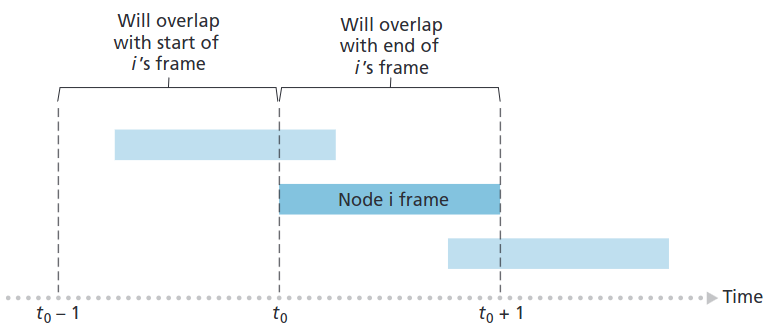
\includegraphics[width = 0.75\linewidth]{img/5/vulnerability.png}
    \caption{Pure ALOHA vulnerability window. The \textbf{vulnerable period} is $T = 2L/R$---two frame times!}
    \label{fig:ALOHA-puro-vulnerability}
\end{figure}

\clearpage
\noindent \textbf{Slotted ALOHA:}\\[2pt]
\noindent With \underline{slotted} ALOHA we'll assume the following:
\begin{itemize}[nolistsep,noitemsep] \small
    \item \underline{Time is divided into slots} of size $L/R$ (a slot equals the time to transmit one frame).
    \item Nodes start to \underline{transmit frames only at the beginnings of slots}.
    \item The nodes are synchronized so that each node knows when the slots begin.
    \item If two or more frames collide in a slot, then all the nodes detect the collision event before the slot ends.
\end{itemize}

\vspace{0.5em}
\noindent The operations of slotted ALOHA are the following:
\begin{itemize}
    \item When the node has a fresh frame to send, it waits until the beginning of the next slot and transmits the entire frame in the slot.
    
    \item If there isn’t a collision, the node has successfully transmitted its frame and thus need not consider retransmitting the frame. (The node can prepare a new frame for transmission, if it has one.)
    
    \item If there is a collision, the node detects the collision before the end of the slot. The node retransmits its frame in each subsequent slot with probability $p$ until the frame is transmitted without a collision (as in, the node effectively tosses a biased coin; the event heads corresponds to "retransmit", which occurs with probability $p$.).
\end{itemize}

\begin{figure}[H]
    \centering
    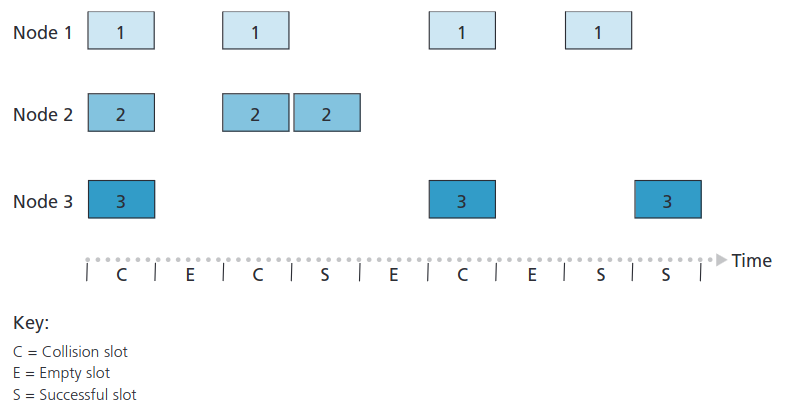
\includegraphics[width = 0.75\linewidth]{img/5/ALOHA.png}
    \caption{Collision visualization in ALOHA protocol}
    \label{fig:ALOHA}
\end{figure}

\noindent\textbf{Efficiency Comparison:}\mbox{}\\[2pt]
\noindent Definindo a utilização do canal como:
$$
    S(G) = G e^{-\alpha G}\; \text{em que}\; \alpha\; \propto\; \text{período de vulnerabilidade}
$$

\vspace{-1em}
\begin{figure}[H]
    \centering
    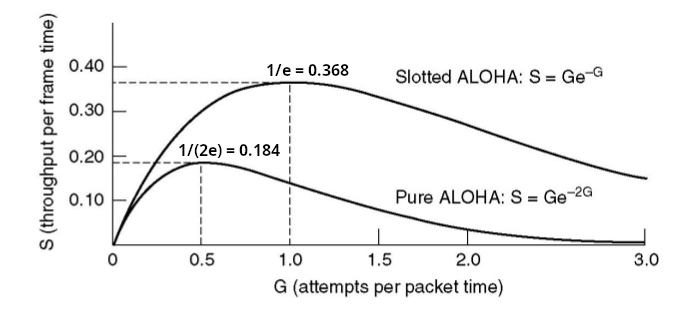
\includegraphics[width = 0.7\linewidth]{img/5/Efficiency-ALOHA.png}
    \caption{ALOHA protocols---efficiency comparison.}
    \label{fig:efficiency-ALOHA}
\end{figure}

%//==============================--@--==============================//%
\newpage
\paragraph[5.3.2.2 CSMA (Carrier Sense Multiple Access)]{$\pmb{\star}$ CSMA (Carrier Sense Multiple Access)}\mbox{}\\[4pt]
In CSMA, a node’s decision to transmit takes into account the activity of other nodes attached to the broadcast channel, unlike ALOHA protocols. Two important rules for CSMA are:

\begin{enumerate}
    \item \textbf{Listen before speaking}: This is called carrier sensing, where a node listens to the channel before transmitting. If a frame from another node is being transmitted, the node waits until no transmissions are detected and then begins transmission.
    \item \textbf{Stop talking if someone else begins talking}: In networking, this is called collision detection. A transmitting node listens to the channel while it is trans- mitting. If it detects an interfering frame, it stops transmitting and waits a random amount of time before repeating the sense-and-transmit-when-idle cycle.
\end{enumerate}

\noindent Collisions can still occur in CSMA despite carrier sensing. Consider four nodes (A, B, C, D) attached to a linear broadcast bus. At time $t_0$, node B senses the channel is idle and begins transmitting. The bits propagate in both directions along the broadcast medium. At time $t_1\: (t_1 > t_0)$, node D has a frame to send. Even though B is transmitting, the bits haven't reached D yet, so D senses the channel idle at $t_1$. In accordance with the CSMA protocol, D begins transmitting, and shortly after, B's transmission interferes with D's transmission at D. It is evident that the end-to-end channel propagation delay plays a crucial role in determining the performance of a broadcast channel.

%//==============================--@--==============================//%
\paragraph[5.3.2.3 CSMA/CD (Carrier Sense Multiple Access with Collision Detection)]{$\pmb{\star}$ CSMA/CD (Carrier Sense Multiple Access with Collision Detection)}\mbox{}\\[4pt]
CSMA/CD improves upon CSMA by incorporating collision detection. Nodes abort their transmission shortly after detecting a collision, thus reducing wasted channel time. The operation of CSMA/CD from the perspective of a node's adapter is as follows:

\begin{enumerate}
    \item Obtain datagram, prepare link-layer frame, put frame in adapter buffer.
    \item Sense channel idle or busy; if idle, transmit frame; if busy, wait until no signal energy detected and transmit.
    \item Monitor for signal energy from other adapters while transmitting.
    \item If no signal energy detected during transmission, frame is complete; if signal energy detected, abort transmission.
    \item Enter the exponential backoff state after aborting and return to step 2.
\end{enumerate}

\noindent \textbf{Binary Exponential Backoff:} $\boxed{ t_\text{backoff} = K \cdot t_\text{frame} }$\\[2pt]
This algorithm addresses the problem of choosing an appropriate random backoff time interval by adapting the range of values based on the number of collisions experienced by a frame. When a frame has undergone $n$ collisions, the algorithm selects the value of $K$ randomly from $\{0, \dots, 2^{n} - 1\}$. The maximum value for $n$ is usually limited to 10 to prevent excessive waiting times.

\vspace{1em}
\noindent \textbf{CSMA/CD Efficiency:}\\[2pt]
Efficiency is defined as the long-run fraction of time during which frames are being transmitted without collisions when there is a large number of active nodes with many frames to send. Let $d_{prop}$ be the maximum signal energy propagation time between two adapters, and $d_{trans}$ be the time to transmit a maximum-size frame. The efficiency approximation is:
$$
    \text{Efficiency} = \frac{1}{1 + 5\, d_{prop}/d_{trans}}
$$

%//==============================--@--==============================//%
\paragraph[5.3.2.4 CSMA/CA (Carrier Sense Multiple Access with Collision Avoidance)]{$\pmb{\star}$ CSMA/CA (Carrier Sense Multiple Access with Collision Avoidance)}\mbox{}\\[4pt]
CSMA/CA is an improvement to the CSMA protocol that focuses on collision avoidance. It is commonly used in wireless networks like Wi-Fi, where collision detection is not feasible due to hardware limitations and issues like the hidden terminal problem and fading. In wireless LANs, such as 802.11, CSMA/CA employs a random access protocol with a distributed coordination function (DCF) and incorporates inter-frame spacing intervals, such as \textbf{Distributed Inter-frame Space (DIFS)} and \textbf{Short Inter-frame Space (SIFS)}.

\begin{enumerate}
    \item If the station senses the channel idle initially, it transmits its frame after a short period of time known as the Distributed Inter-frame Space (DIFS).
    \item Otherwise, the station chooses a random backoff value using binary exponential backoff (as discussed earlier) and counts down this value after DIFS when the channel is sensed idle. The counter value remains frozen while the channel is sensed busy.
    \item When the counter reaches zero (which can only occur while the channel is sensed idle), the station transmits the entire frame and then waits for an acknowledgment.
    \item If an acknowledgment is received, the transmitting station knows that its frame has been correctly received at the destination station.
    \begin{enumerate}
        \item If the station has another frame to send, it begins the protocol at step 2.
        \item If the acknowledgment isn't received, the transmitting station reenters the backoff phase in step 2, with the random value chosen from a larger interval.
    \end{enumerate}
\end{enumerate}

\begin{figure}[H]
    \centering
    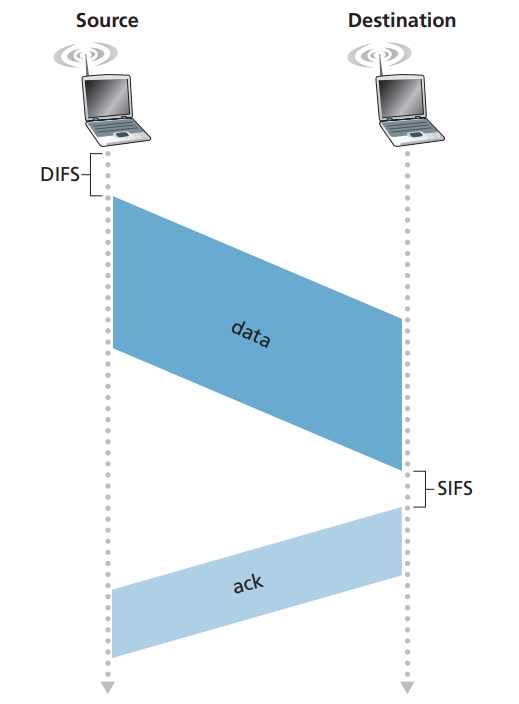
\includegraphics[width = 0.55\linewidth]{img/5/link-layer-ack.png}
    \caption{Link-layer acknowledgments \cite{Kurose2017}}
    \label{fig:link-layer-ack}
\end{figure}

%//==============================--@--==============================//%
\paragraph[5.3.2.5 RTS-CTS (Request to Send - Clear to Send)]{$\pmb{\star}$ RTS-CTS (Request to Send - Clear to Send)}\mbox{}\\[4pt]
RTS-CTS is a mechanism used in conjunction with CSMA/CA to further reduce collisions in wireless networks, especially in the presence of hidden terminals. 

\begin{theo}[\underline{Hidden terminal}]{def:hidden-terminal}\label{def:hidden-terminal}
    The hidden terminal problem occurs when multiple wireless stations within the range of an access point (AP) are unable to detect each other's signals due to limited signal ranges. This situation results in collisions and wasted channel resources, as stations might transmit frames unknowingly during another station's ongoing transmission to the AP.
    
    To tackle this problem, the IEEE 802.11 protocol introduces the use of short RTS and CTS control frames to reserve channel access. The sender transmits a \textbf{Request to Send (RTS)} packet to the receiver, which replies with a \textbf{Clear to Send (CTS)} packet. Neighboring nodes overhearing the RTS or CTS packets update their Network Allocation Vector, helping them anticipate when the channel will be available again.
\end{theo}

\noindent The steps for RTS-CTS are:
\begin{enumerate}
    \item The sender senses the channel to check if it is idle before initiating the transmission process.
    \item The sender prepares to transmit a frame and sends an RTS packet to the receiver, specifying the total time required to transmit the frame and its acknowledgment.
    \item The receiver, upon receiving the RTS packet, responds with a CTS packet, which confirms its readiness and reserves the channel for the specified duration.
    \item Neighboring nodes that overhear the RTS or CTS packets update their Network Allocation Vector (NAV) to determine when the channel will be free again and defer their transmissions accordingly.
    \item The sender waits for the CTS packet; if received, it proceeds to transmit the frame.
    \item If the sender does not receive the CTS packet, it performs a binary exponential backoff and retries the process from step 1.
    \item Once the frame is successfully transmitted, the receiver sends an ACK packet to the sender to confirm successful reception.
    \item Other nodes that overhear the ACK packet can also update their NAV and defer their transmissions accordingly.
\end{enumerate}

\noindent By employing the RTS-CTS mechanism, nodes reserve the channel, effectively notifying other nodes of ongoing transmissions. This helps to reduce collisions and address the hidden terminal problem. However, the RTS-CTS exchange can introduce additional delay and consume channel resources.

To strike a balance between collision avoidance and performance, the RTS-CTS mechanism is typically only used for reserving the channel for long \texttt{DATA} frames. In practice, wireless stations can set an RTS threshold, activating the RTS-CTS sequence only for frames exceeding the threshold. Many wireless stations adopt a default RTS threshold value larger than the maximum frame length, effectively skipping the RTS-CTS sequence for all \texttt{DATA} frames sent, optimizing resource usage and minimizing delay.

%//==============================--@--==============================//%
\clearpage
\subsubsection[5.3.3 Taking-Turns Protocols]{$\rightarrow$ Taking-Turns Protocols}
\label{subsec:turn-access-protocols}

Taking-turns protocols, such as polling and token-passing protocols, aim to improve throughput and reduce collisions.

%//==============================--@--==============================//%
\paragraph[5.3.3.1 Polling Protocol]{$\pmb{\star}$ Polling Protocol}\mbox{}\\[4pt]
A master node polls other nodes in a round-robin\footnotemark[5] fashion, allowing them to transmit up to a maximum number of frames. This method eliminates collisions and empty slots, resulting in higher efficiency. However, it introduces polling delay and risks a single point of failure with the master node.

\vspace{1em}
\noindent \textbf{Example:} Bluetooth Protocol
\begin{enumerate}
    \item A master node (e.g., a Bluetooth headset) establishes connections with one or more slave nodes (e.g., a smartphone and a tablet).
    \item The master node polls each slave node, granting them permission to transmit data for a limited time.
    \item After a slave node has transmitted its data, the master node polls the next slave node in the sequence.
    \item This process continues in a cyclic manner, enabling communication between the master and slave nodes.
\end{enumerate}

%//==============================--@--==============================//%
\paragraph[5.3.3.2 Token-Passing Protocol]{$\pmb{\star}$ Token-Passing Protocol}\mbox{}\\[4pt]
In token-passing protocols, a special-purpose frame (the token) is exchanged among nodes in a fixed order. A node holding the token can transmit frames before passing the token to the next node. This method is decentralized and efficient, but may face issues related to node failure or token circulation.

\vspace{1em}
\noindent \textbf{Example:} IEEE 802.5 Token Ring Protocol
\begin{enumerate}
    \item Nodes are organized in a logical ring topology, with each node connected to its two neighboring nodes.
    \item The token, a special-purpose frame, circulates through the ring.
    \item When a node receives the token and has data to transmit, it replaces the token with its data frame and sends it along the ring.
    \item As the data frame traverses the ring, the destination node reads the data and marks the frame as acknowledged.
    \item The frame eventually returns to the source node, which then removes the frame from the ring and releases a new token for circulation.
    \item If a node receives the token but has no data to transmit, it forwards the token to the next node in the ring.
\end{enumerate}

\footnotetext[5]{%
    In the context of polling protocols, round-robin refers to the method of visiting each node in a predefined cyclic sequence, ensuring that each node gets an opportunity to transmit data in a fair manner.
}

%//==============================--@--===========================//%